% Options for packages loaded elsewhere
\PassOptionsToPackage{unicode}{hyperref}
\PassOptionsToPackage{hyphens}{url}
\PassOptionsToPackage{dvipsnames,svgnames,x11names}{xcolor}
%
\documentclass[
  letterpaper,
  DIV=11,
  numbers=noendperiod]{scrartcl}

\usepackage{amsmath,amssymb}
\usepackage{iftex}
\ifPDFTeX
  \usepackage[T1]{fontenc}
  \usepackage[utf8]{inputenc}
  \usepackage{textcomp} % provide euro and other symbols
\else % if luatex or xetex
  \usepackage{unicode-math}
  \defaultfontfeatures{Scale=MatchLowercase}
  \defaultfontfeatures[\rmfamily]{Ligatures=TeX,Scale=1}
\fi
\usepackage{lmodern}
\ifPDFTeX\else  
    % xetex/luatex font selection
\fi
% Use upquote if available, for straight quotes in verbatim environments
\IfFileExists{upquote.sty}{\usepackage{upquote}}{}
\IfFileExists{microtype.sty}{% use microtype if available
  \usepackage[]{microtype}
  \UseMicrotypeSet[protrusion]{basicmath} % disable protrusion for tt fonts
}{}
\makeatletter
\@ifundefined{KOMAClassName}{% if non-KOMA class
  \IfFileExists{parskip.sty}{%
    \usepackage{parskip}
  }{% else
    \setlength{\parindent}{0pt}
    \setlength{\parskip}{6pt plus 2pt minus 1pt}}
}{% if KOMA class
  \KOMAoptions{parskip=half}}
\makeatother
\usepackage{xcolor}
\usepackage[top=30mm,left=20mm,heightrounded]{geometry}
\setlength{\emergencystretch}{3em} % prevent overfull lines
\setcounter{secnumdepth}{3}
% Make \paragraph and \subparagraph free-standing
\makeatletter
\ifx\paragraph\undefined\else
  \let\oldparagraph\paragraph
  \renewcommand{\paragraph}{
    \@ifstar
      \xxxParagraphStar
      \xxxParagraphNoStar
  }
  \newcommand{\xxxParagraphStar}[1]{\oldparagraph*{#1}\mbox{}}
  \newcommand{\xxxParagraphNoStar}[1]{\oldparagraph{#1}\mbox{}}
\fi
\ifx\subparagraph\undefined\else
  \let\oldsubparagraph\subparagraph
  \renewcommand{\subparagraph}{
    \@ifstar
      \xxxSubParagraphStar
      \xxxSubParagraphNoStar
  }
  \newcommand{\xxxSubParagraphStar}[1]{\oldsubparagraph*{#1}\mbox{}}
  \newcommand{\xxxSubParagraphNoStar}[1]{\oldsubparagraph{#1}\mbox{}}
\fi
\makeatother


\providecommand{\tightlist}{%
  \setlength{\itemsep}{0pt}\setlength{\parskip}{0pt}}\usepackage{longtable,booktabs,array}
\usepackage{calc} % for calculating minipage widths
% Correct order of tables after \paragraph or \subparagraph
\usepackage{etoolbox}
\makeatletter
\patchcmd\longtable{\par}{\if@noskipsec\mbox{}\fi\par}{}{}
\makeatother
% Allow footnotes in longtable head/foot
\IfFileExists{footnotehyper.sty}{\usepackage{footnotehyper}}{\usepackage{footnote}}
\makesavenoteenv{longtable}
\usepackage{graphicx}
\makeatletter
\newsavebox\pandoc@box
\newcommand*\pandocbounded[1]{% scales image to fit in text height/width
  \sbox\pandoc@box{#1}%
  \Gscale@div\@tempa{\textheight}{\dimexpr\ht\pandoc@box+\dp\pandoc@box\relax}%
  \Gscale@div\@tempb{\linewidth}{\wd\pandoc@box}%
  \ifdim\@tempb\p@<\@tempa\p@\let\@tempa\@tempb\fi% select the smaller of both
  \ifdim\@tempa\p@<\p@\scalebox{\@tempa}{\usebox\pandoc@box}%
  \else\usebox{\pandoc@box}%
  \fi%
}
% Set default figure placement to htbp
\def\fps@figure{htbp}
\makeatother

\KOMAoption{captions}{tableheading}
\makeatletter
\@ifpackageloaded{caption}{}{\usepackage{caption}}
\AtBeginDocument{%
\ifdefined\contentsname
  \renewcommand*\contentsname{Table of contents}
\else
  \newcommand\contentsname{Table of contents}
\fi
\ifdefined\listfigurename
  \renewcommand*\listfigurename{List of Figures}
\else
  \newcommand\listfigurename{List of Figures}
\fi
\ifdefined\listtablename
  \renewcommand*\listtablename{List of Tables}
\else
  \newcommand\listtablename{List of Tables}
\fi
\ifdefined\figurename
  \renewcommand*\figurename{Figure}
\else
  \newcommand\figurename{Figure}
\fi
\ifdefined\tablename
  \renewcommand*\tablename{Table}
\else
  \newcommand\tablename{Table}
\fi
}
\@ifpackageloaded{float}{}{\usepackage{float}}
\floatstyle{ruled}
\@ifundefined{c@chapter}{\newfloat{codelisting}{h}{lop}}{\newfloat{codelisting}{h}{lop}[chapter]}
\floatname{codelisting}{Listing}
\newcommand*\listoflistings{\listof{codelisting}{List of Listings}}
\makeatother
\makeatletter
\makeatother
\makeatletter
\@ifpackageloaded{caption}{}{\usepackage{caption}}
\@ifpackageloaded{subcaption}{}{\usepackage{subcaption}}
\makeatother

\usepackage{bookmark}

\IfFileExists{xurl.sty}{\usepackage{xurl}}{} % add URL line breaks if available
\urlstyle{same} % disable monospaced font for URLs
\hypersetup{
  pdftitle={Standard Data Science Template},
  pdfauthor={Analytics Team},
  colorlinks=true,
  linkcolor={blue},
  filecolor={Maroon},
  citecolor={Blue},
  urlcolor={Blue},
  pdfcreator={LaTeX via pandoc}}


\title{Standard Data Science Template}
\usepackage{etoolbox}
\makeatletter
\providecommand{\subtitle}[1]{% add subtitle to \maketitle
  \apptocmd{\@title}{\par {\large #1 \par}}{}{}
}
\makeatother
\subtitle{Project Template}
\author{Analytics Team}
\date{2023-01-01}

\begin{document}
\maketitle

\renewcommand*\contentsname{Table of contents}
{
\hypersetup{linkcolor=}
\setcounter{tocdepth}{2}
\tableofcontents
}

\newpage{}

\section{Introduction}\label{introduction}

Describe the dataset.

\section{Problem Statement}\label{problem-statement}

Describe the problem. What are we trying to predict? Is there a baseline
to measure against? Does prediction bring value? ``So what?''

\section{Exploratory Data Analysis}\label{exploratory-data-analysis}

\begin{enumerate}
\def\labelenumi{\arabic{enumi}.}
\tightlist
\item
  Profile the dataset.
\end{enumerate}

Check for correct data types, nulls, uniqueness, granularity and top
value counts.

\begin{longtable}[]{@{}llllll@{}}
\caption{Quality Check of All Fields}\tabularnewline
\toprule\noalign{}
& Data Type & Mode & Mode \% of total & Unique Count & Percent Null \\
\midrule\noalign{}
\endfirsthead
\toprule\noalign{}
& Data Type & Mode & Mode \% of total & Unique Count & Percent Null \\
\midrule\noalign{}
\endhead
\bottomrule\noalign{}
\endlastfoot
Age & Float & 24.0 & 4\% & 88 & 20\% \\
Fare & Float & 8.05 & 5\% & 248 & 0\% \\
Survived & Integer & 0 & 62\% & 2 & 0\% \\
Pclass & Integer & 3 & 55\% & 3 & 0\% \\
SibSp & Integer & 0 & 68\% & 7 & 0\% \\
Parch & Integer & 0 & 76\% & 7 & 0\% \\
Name & String & Dooley, Mr. Patrick & 0\% & 891 & 0\% \\
Sex & String & male & 65\% & 2 & 0\% \\
Ticket & String & 347082 & 1\% & 681 & 0\% \\
Cabin & String & G6 & 2\% & 147 & 77\% \\
Embarked & String & S & 72\% & 3 & 0\% \\
\end{longtable}

\begin{enumerate}
\def\labelenumi{\arabic{enumi})}
\setcounter{enumi}{1}
\tightlist
\item
  Compute descriptive statistics of numeric fields.
\end{enumerate}

\begin{longtable}[]{@{}lllllll@{}}
\caption{Descriptive Statistics of Numeric Fields}\tabularnewline
\toprule\noalign{}
& Min & Mean & Median & Max & Standard Dev & Kurtosis \\
\midrule\noalign{}
\endfirsthead
\toprule\noalign{}
& Min & Mean & Median & Max & Standard Dev & Kurtosis \\
\midrule\noalign{}
\endhead
\bottomrule\noalign{}
\endlastfoot
Survived & 0 & 0.4 & 0.0 & 1 & 0.5 & -1.8 \\
Pclass & 1 & 2.3 & 3.0 & 3 & 0.8 & -1.3 \\
Age & 0 & 29.7 & 28.0 & 80 & 14.5 & 0.2 \\
SibSp & 0 & 0.5 & 0.0 & 8 & 1.1 & 17.9 \\
Parch & 0 & 0.4 & 0.0 & 6 & 0.8 & 9.8 \\
Fare & 0 & 32.2 & 14.5 & 512 & 49.7 & 33.4 \\
\end{longtable}

\begin{enumerate}
\def\labelenumi{\arabic{enumi})}
\setcounter{enumi}{2}
\tightlist
\item
  Explore dependent variable
\end{enumerate}

Not necessary, as it is binary. Accomplished above.

\begin{enumerate}
\def\labelenumi{\arabic{enumi})}
\setcounter{enumi}{3}
\tightlist
\item
  Visualize independent variables.
\end{enumerate}

\begin{figure}[H]

{\centering \pandocbounded{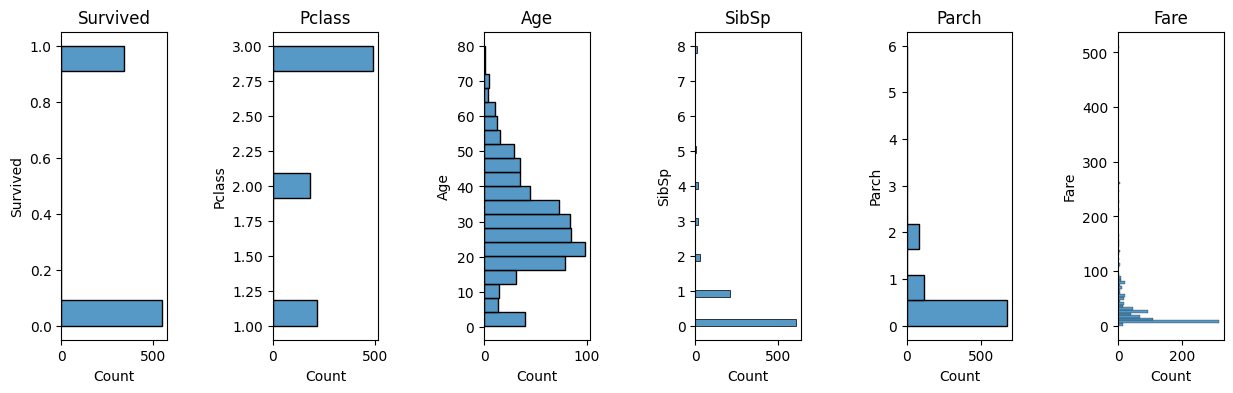
\includegraphics[keepaspectratio]{Titanic_Classification_Report_files/figure-pdf/cell-6-output-1.png}}

}

\caption{Distribution of Numeric Fields}

\end{figure}%

\begin{enumerate}
\def\labelenumi{\arabic{enumi})}
\setcounter{enumi}{4}
\tightlist
\item
  Explore relationship independent variables have on dependent variable.

  \begin{itemize}
  \tightlist
  \item
    Correlations
  \item
    Predictive Power Scores
  \end{itemize}
\end{enumerate}

\begin{figure}[H]

{\centering \pandocbounded{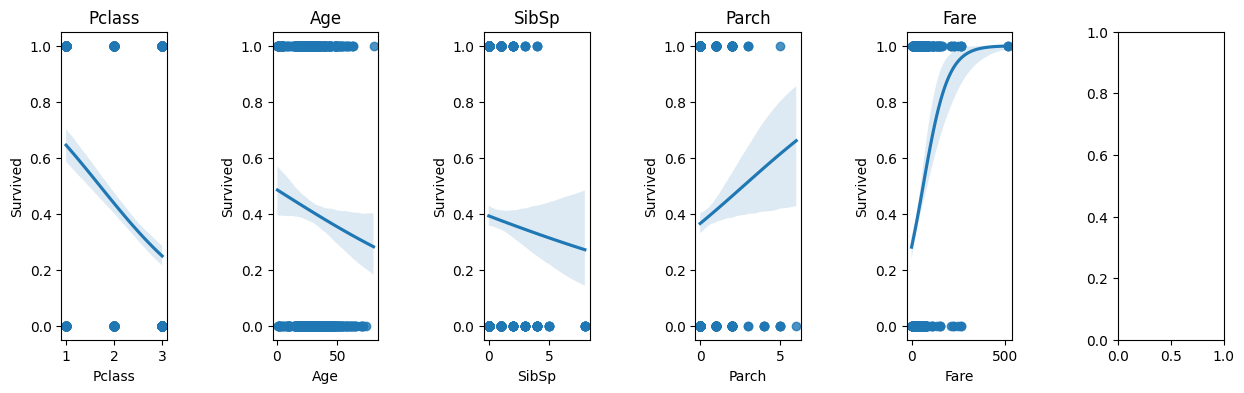
\includegraphics[keepaspectratio]{Titanic_Classification_Report_files/figure-pdf/cell-7-output-1.png}}

}

\caption{Relationship Between Numeric Fields and Target}

\end{figure}%

\begin{figure}[H]

{\centering \pandocbounded{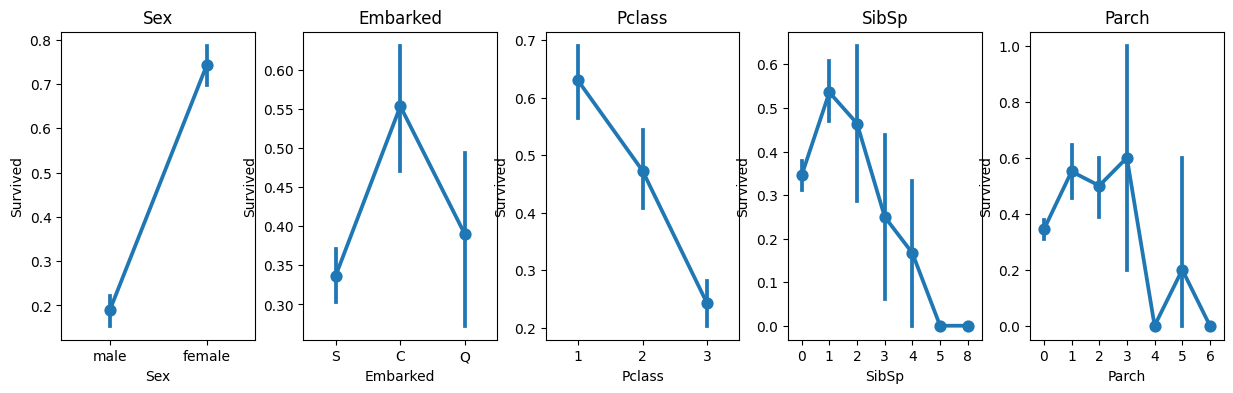
\includegraphics[keepaspectratio]{Titanic_Classification_Report_files/figure-pdf/cell-8-output-1.png}}

}

\caption{Relationship between Categorical Fields and Target}

\end{figure}%

\begin{verbatim}
Unable to display output for mime type(s): application/vnd.plotly.v1+json
\end{verbatim}

Parallel categories plot with respect to target

\begin{verbatim}
Unable to display output for mime type(s): application/vnd.plotly.v1+json
\end{verbatim}

Parallel coordinates plot with respect to target

\begin{figure}[H]

{\centering \pandocbounded{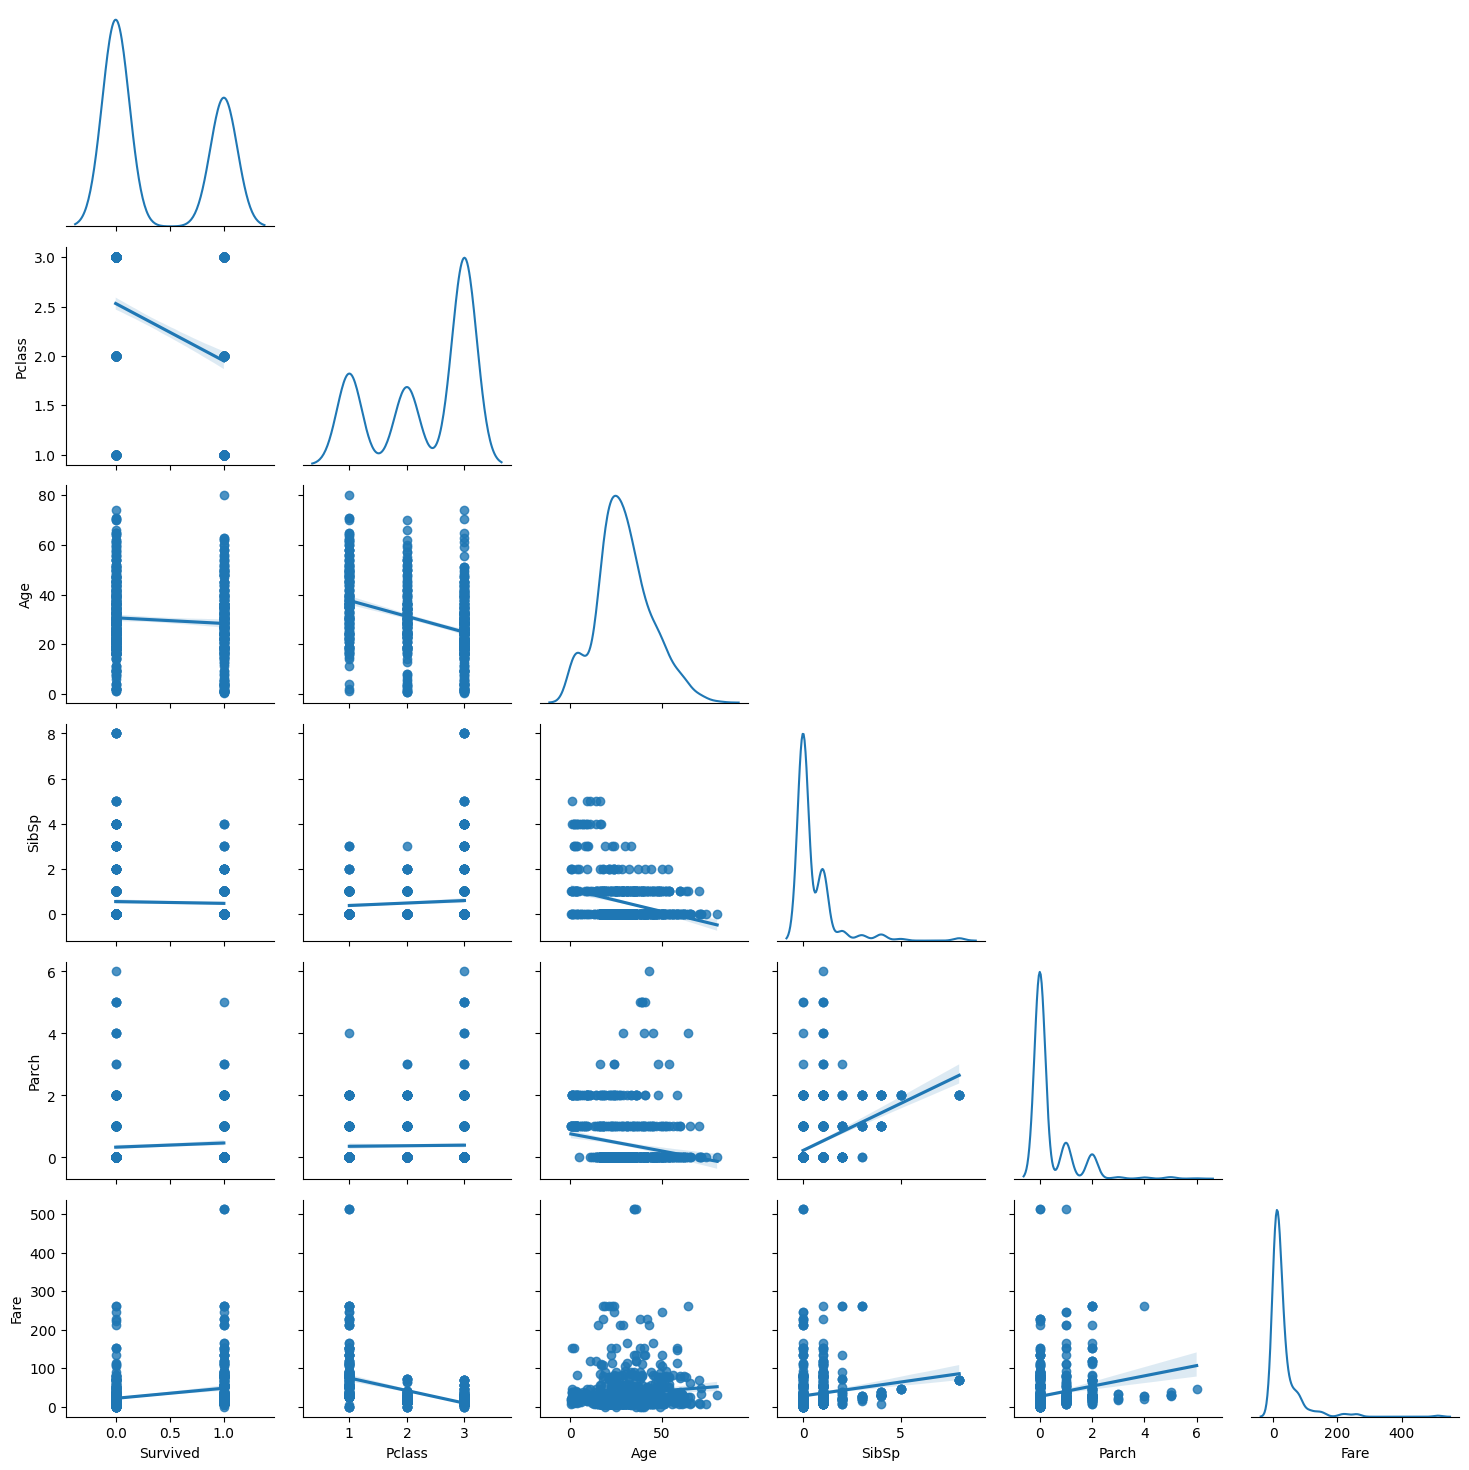
\includegraphics[keepaspectratio]{Titanic_Classification_Report_files/figure-pdf/cell-12-output-1.png}}

}

\caption{Relationships Between Numeric Fields}

\end{figure}%

\section{Feature Engineering}\label{feature-engineering}

Should we remove outliers? manually impute nulls? handle
high-value-count categories? handle date or time columns? convert data
types?

Select a specific set of features and optionally re-name them.

\section{Model Selection}\label{model-selection}

Run autoML to train the model. This can be for either regression or
classification, but the focus her will be for regression and clustering

\section{Analysis of Feature
Relationships}\label{analysis-of-feature-relationships}

Calculate shap values for the model and visualize them with respect to
each feature

Look at pair plot and parallel coordinates (plotly or hiplot)

\section{Model Tuning}\label{model-tuning}

\section{Model Validation and
Testing}\label{model-validation-and-testing}

\section{Results}\label{results}

\section{Conclusion}\label{conclusion}

\section{Appendix}\label{appendix}

\section{Example PDF Usage \&
Formatting}\label{example-pdf-usage-formatting}

\begin{itemize}
\item
  Jupyter cell behaviour:

  \begin{itemize}
  \item
    the following code can be added to the top of a cell to change how
    it renders in the PDF
  \item
    toggle output

    \begin{itemize}
    \tightlist
    \item
      \#\textbar{} output: false
    \item
      \#\textbar{} output: true
    \end{itemize}
  \item
    Toggle code in output

    \begin{itemize}
    \tightlist
    \item
      \#\textbar{} echo: false (default)
    \item
      \#\textbar{} echo: true
    \end{itemize}
  \end{itemize}
\item
  add captions to an output
\item
  \#\textbar{} fig-cap: caption for plot
\item
  \#\textbar{} tbl-cap: caption for table
\item
  \href{https://quarto.org/docs/reference/cells/cells-jupyter.html}{more
  documentation here}
\item
  Plotly visualization shortcuts code shortcuts:

  \begin{itemize}
  \tightlist
  \item
    px-fig - Create over 30 types of statistical and scientific graphics
    figures.
  \item
    px-update - Update layout and data trace styling of existing figure.
  \item
    px-args - Select arguments from lists of options to modify figure
    styling.
  \end{itemize}
\end{itemize}




\end{document}
